\begin{block}{Partitions interactives}
\begin{figure}
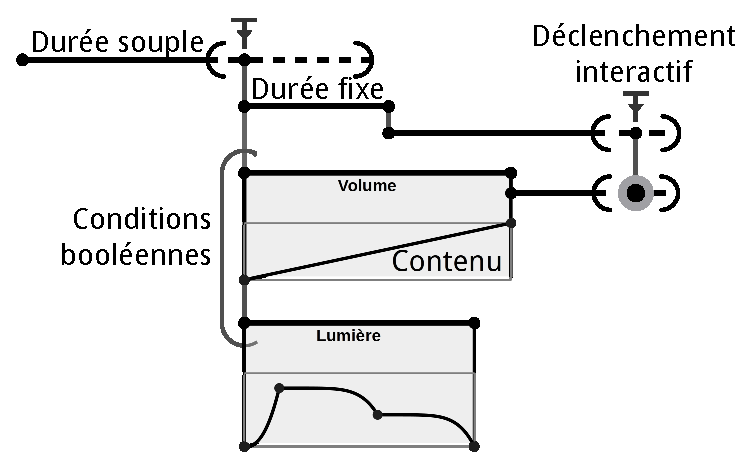
\includegraphics[width=\columnwidth]{images/score.eps}
\caption{Syntaxe d'une partition interactive}
\end{figure}
Possibilités d'écritures forment un langage de programmation structuré axé sur l'organisation temporelle. 
\textbf{Boucles} et \textbf{hiérarchie}, calcul possible via \textbf{Javascript}.
Applications : musique interactive, scénographie et spectacle vivant, contrôle de robots.
Autres approches graphiques : \textbf{OpenMusic}~\cite{bresson_openmusic:_2011}, \textbf{Antescofo}~\cite{cont2008antescofo}, \textbf{INscore}~\cite{fober2012environment}; ainsi qu'approches programmatiques : \textbf{Abjad}, \textbf{Tuiles réactives}, \dots
\end{block}